% generated by experiments/build_paper_assets.py -- do not edit by hand
\begin{figure}[t]
\centering
\resizebox{\linewidth}{!}{%
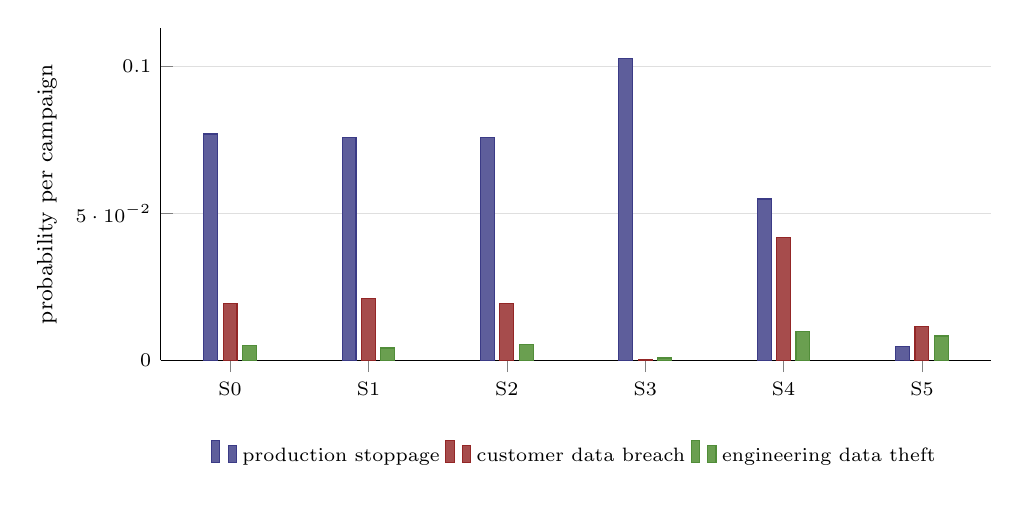
\begin{tikzpicture}
\begin{axis}[
    ybar, width=\linewidth, height=5.8cm,
    ylabel={probability per campaign},
    symbolic x coords={S0,S1,S2,S3,S4,S5}, xtick=data,
    ymin=0, bar width=5pt, enlarge x limits=0.10,
    legend style={at={(0.5,-0.22)}, anchor=north, legend columns=3, font=\scriptsize,
                   draw=none},
    ticklabel style={font=\scriptsize}, label style={font=\footnotesize},
    ymajorgrids, grid style={gray!25}, axis lines*=left,
]
\addplot[fill=MidnightBlue!70, draw=MidnightBlue!85] coordinates {(S0,0.077) (S1,0.0757) (S2,0.0758) (S3,0.1027) (S4,0.0549) (S5,0.0047)};
\addplot[fill=Maroon!70, draw=Maroon!85] coordinates {(S0,0.0192) (S1,0.0209) (S2,0.0193) (S3,0.0003) (S4,0.0418) (S5,0.0116)};
\addplot[fill=OliveGreen!70, draw=OliveGreen!85] coordinates {(S0,0.005) (S1,0.0042) (S2,0.0054) (S3,0.0008) (S4,0.0097) (S5,0.0083)};
\legend{production stoppage, customer data breach, engineering data theft}
\end{axis}
\end{tikzpicture}}
\caption{Consequence mix per campaign under each control scenario, big-game ransomware profile. $S_3$ removes the cheap data-theft outcomes and the production-stoppage probability rises: the displacement effect of section~VI.D made visible.}
\label{fig:mix}
\end{figure}
